
%(BEGIN_QUESTION)
% Copyright 2003, Tony R. Kuphaldt, released under the Creative Commons Attribution License (v 1.0)
% This means you may do almost anything with this work of mine, so long as you give me proper credit

A balanced, three-phase power system has a line voltage of 13.8 kV volts and a line current of 150 amps.  How much power is being delivered to the load (assuming a power factor of 1)?

$$\includegraphics[width=15.5cm]{i02297x01.eps}$$

A 13.8 kV single-phase system could be designed to provide the same amount of power to a load, but it would require heavier-gauge (more expensive!) conductors.  Determine the extra percentage of expense in wire cost (based on the weight of the wires) resulting from the use of single-phase instead of three-phase.

$$\includegraphics[width=15.5cm]{i02297x02.eps}$$

\underbar{file i02297}
%(END_QUESTION)





%(BEGIN_ANSWER)

$P_{load} =$ 3.59 MW

\vskip 10pt

Line current in the three-phase system is given as 150 amps.  According to the 2008 edition of the National Electrical Code, this would require a \#4 AWG copper wire (from table 310.21 in NFPA 70).

Line current in the single-phase system is calculated to be 260 amps.  This would require 1/0 copper wire according to the same table in the NEC.

\vskip 10pt

The ratio of three-phase current to single-phase current is $1 \over \sqrt{3}$, which tells us how much smaller the cross-sectional area of the three-phase conductors may be compared to the cross-sectional area of the single-phase conductors.  However, we know the three-phase system requires 3 conductors whereas the single-phase system requires only 2 conductors: an increase in conductor count of $3 \over 2$.  The overall savings in copper realized by three-phase distribution may therefore be calculated by multiplying these two ratios:

$$\left(1 \over \sqrt{3}\right) \left(3 \over 2\right) = 0.866$$

Therefore, a three-phase power system requires just 86.6\% of the copper required by a single-phase power system to convey the same amount of electrical power!

%(END_ANSWER)





%(BEGIN_NOTES)

This question is good for provoking discussion on the practical, cost-saving benefits of three-phase power systems over single-phase.  Your students will have to do some ``review'' research on wire gauges and weights, but the exercise is well worth it.

%INDEX% Electronics review: 3-phase voltage/current/power calculation

%(END_NOTES)


